\section{Position control with active joint torque focus}\label{sec:pas-pos}

As seen in \ref{subsec:DHPFC}, the equations of motion are used to find the desired torques satisfying the desired joint accelerations. However, the equations of motion do not consider that some of the joints are passive and thus joint torques will be assigned to all joints, both passive and active. This is of course an issue since the computed solution relies on the realization of these torques.

\begin{table}[H]
    \centering
    \begin{tabular}{|c|c|c|}
        \hline
        & \textbf{Value} & \textbf{Unit}\\
        \hline \hline
        Number of obstacles & $3$ & \\
        Number of links & $6$ & \\
        $\theta_{2,d}$ & $-0.2$ & $[rad]$ \\
        $\theta_{3,d}$ & $0.2$ & $[rad]$ \\
        First sim.:$[K_{p}, K_{i}]$ & $[3, 0.01]$ &\\
        Second sim.:$[K_{p}, K_{i}]$ & $[1, 0.001]$ &\\
        \hline
    \end{tabular}
    \caption{Simulation configuration for double position control experiment}
    \label{tab:exp_2xp}
\end{table}

This experiment aims at illustrating the difference in just ignoring the passive joint torque commands and in mapping all joint torques over to the active joints. Because the focus is on the position torques $\boldsymbol{\tau}_P$, the link angles by the second and third obstacles are controlled. They are first controlled by using the equations of motion as in (\ref{eq:dhpfc_taup}). Here the torques for the passive joints are simply neglected. The second simulation shows control where all torques are mapped to the active joints, as explained in \ref{subsec:passive-joints}. For this experiment it is simply chosen that the desired values of the active joints should be followed and that the passive joints could take resulting arbitrary values. This is probably not the optimal choice of variables to control, but a method for explicitly determining this has not yet been developed. The matter is discussed further in \ref{subsec:dis-passive-joints}.

\begin{figure}
    \centering
    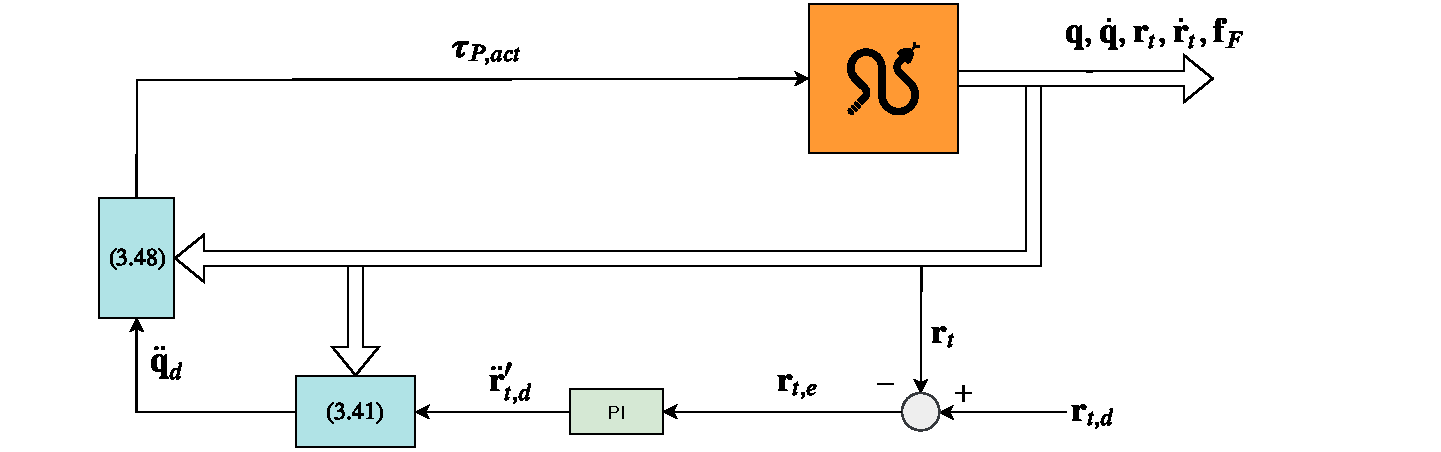
\includegraphics[trim=1cm 0cm 3cm 0cm, clip=true, width=\textwidth]{figures/experiments/control-diagrams/2p-control-diagram.pdf}
    \caption{Control diagram for position control with active joint torque focus}
    \label{fig:diag-2p}
\end{figure}

The minimal CKC formulation is used for both simulations, which implies that the desired angles are defined according to the previous contact point. Further simulation configurations are presented in Table \ref{tab:exp_2xp}. The control structure for the experiment is given in Figure \ref{fig:diag-2p}. The equation (\ref{eq:tau-act}) in the diagram is substituted with (\ref{eq:dhpfc_taup}) for the first simulation.



\subsection{Control torques computed for both passive and active joints}

For this simulation, the control torques from (\ref{eq:dhpfc_taup}) belonging to the active variables were commanded to the snake robot. The rest of the motor torque commands were simply ignored. The resulting torques and contact link angles can be seen in Figure \ref{fig:2xp-1}. The contact link angle $\theta_{t,3}$ settles at a value close to its desired value. However, $\theta_{t,2}$ is very far from reaching its desired value and the control is overall considered unsuccessful.

\begin{figure}[H]
    \centering
    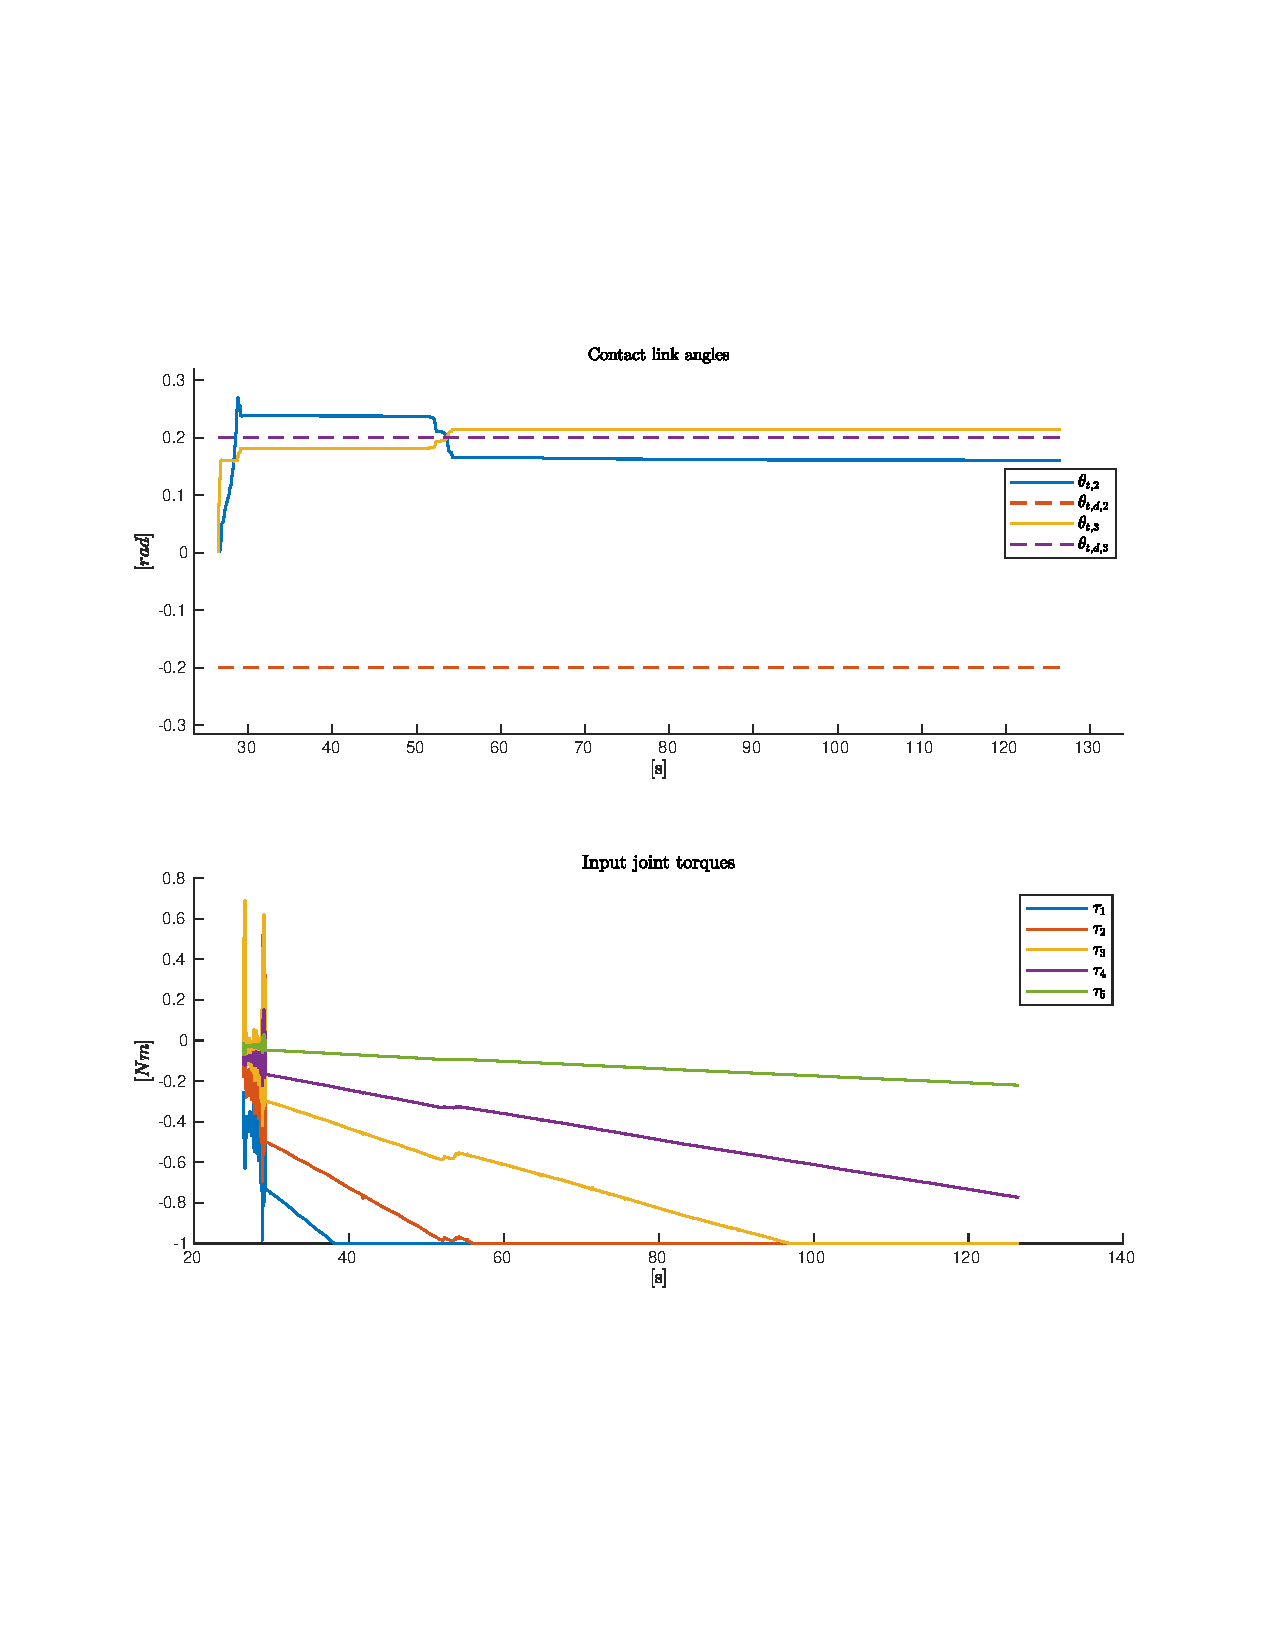
\includegraphics[trim=2.1cm 6cm 2.1cm 5cm, clip=true, width=\textwidth]{figures/experiments/2xpos/2xpos-2plot-fail.pdf}
    \caption{Results from position control experiment with torque calculation for all joints}
    \label{fig:2xp-1}
\end{figure}

From Figure \ref{fig:2xp-1} it can also be observed that the joint torques reach a saturation limit, which is probably the reason for why very little change is noticed in the joint angles. The saturation is in place to keep the snake robot from making large sudden movements that would move it outside of the scope of the model. A higher saturation limit is also tested without further success. Another reason for the static behavior of the angles is the configuration of the snake robot and obstacles, presented in \ref{fig:init-gazebo}. When all applied joint torques are negative the snake robot will try to curve up towards the two right side obstacles. By doing so it is mainly just pushing against the obstacles, much like the experiment in \ref{tab:exp_valid1}. This will logically lead to a jam rather than any movement.

\subsection{Control torques computed for only active joints}

This time all control torques are calculated to be commanded to the active joints, which means that no commands are ignored. The desired passive joint acceleration values are on the other hand ignored. Therefore, this is not an optimal approach either and required a lot of tuning to get it right. The results are presented in Figure \ref{fig:2xp-2}. $\theta_{t,2}$ still deviates slightly from its desired value $\theta_{t,d,2}$, but the performance is considered much better than in the previous simulation.

\begin{figure}
    \centering
    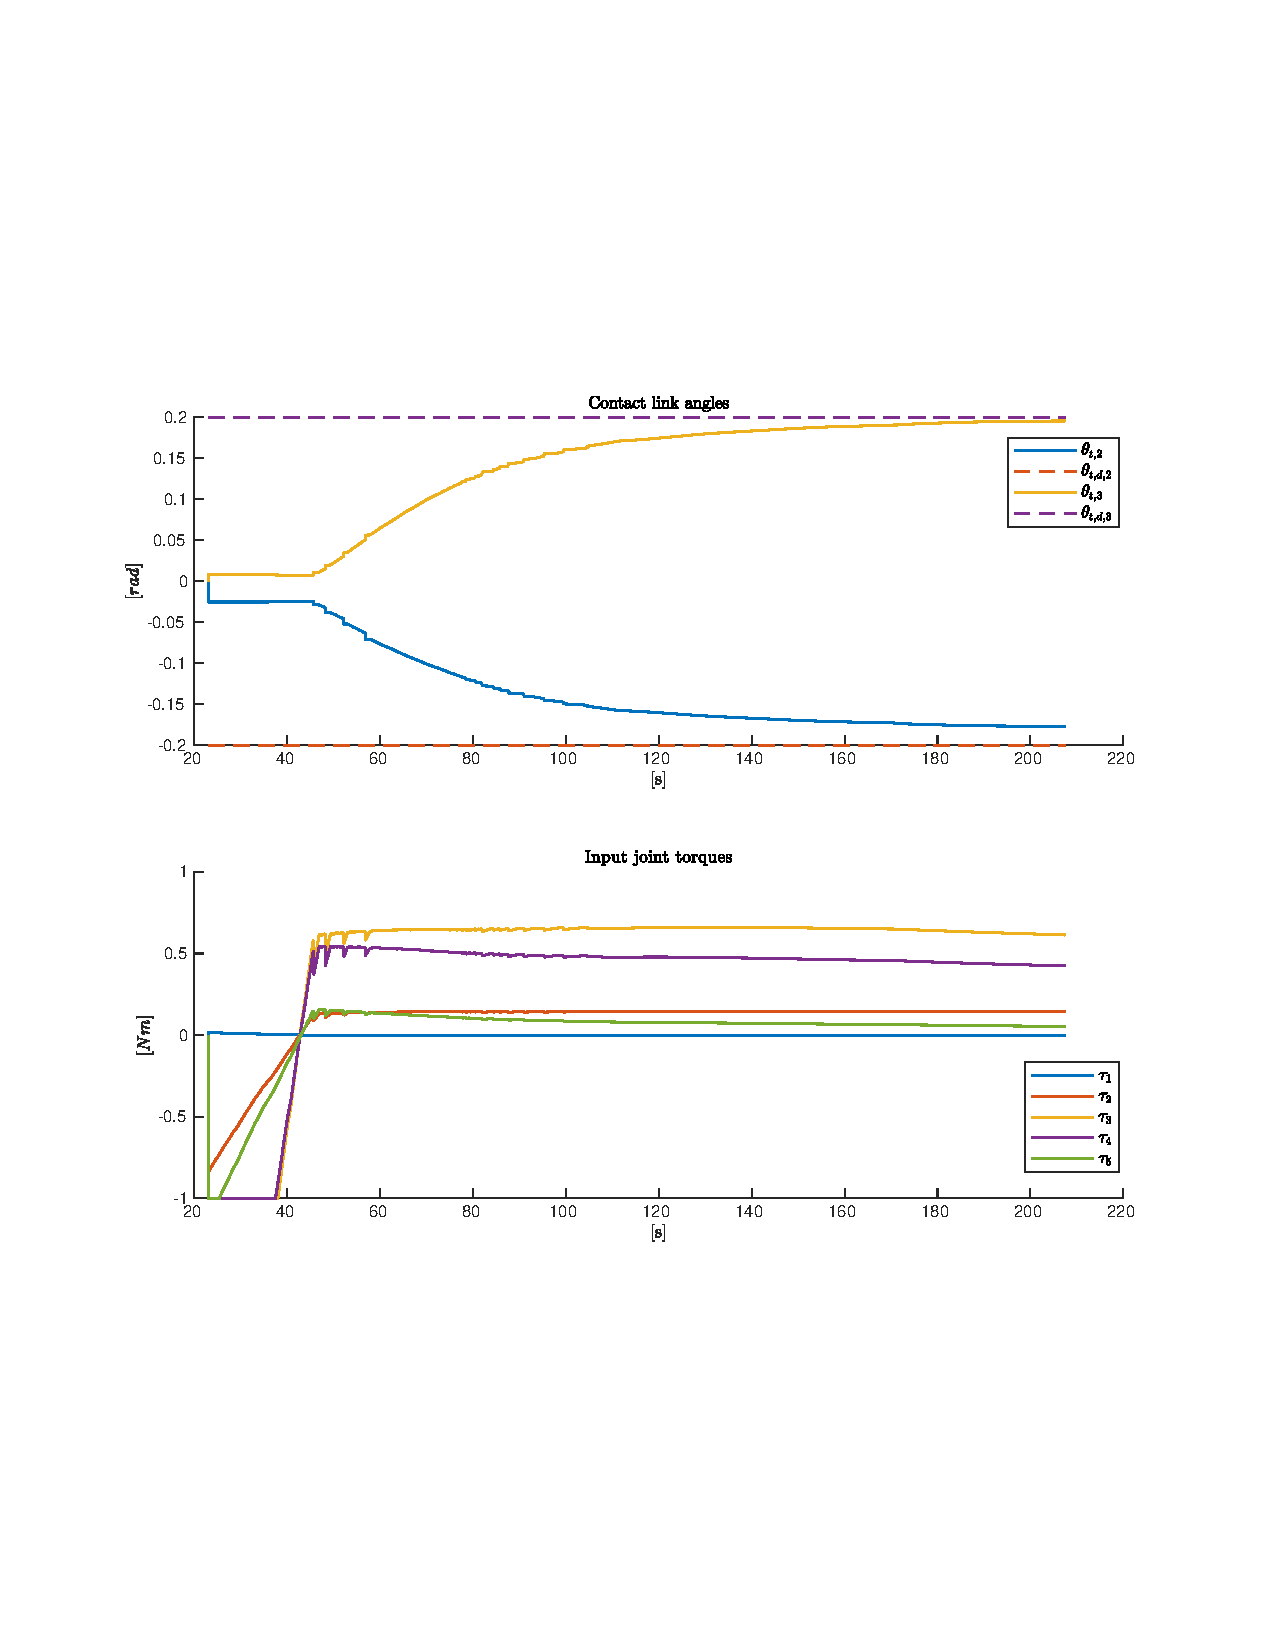
\includegraphics[trim=2.1cm 6cm 2.1cm 6cm, clip=true, width=\textwidth]{figures/experiments/2xpos/2xpos-2plot.pdf}
    \caption{Results from position control experiment with torque calculation for only active joints}
    \label{fig:2xp-2}
\end{figure}

It should be noted that the snake robot is moving quite slowly in both of the simulations. This means that $\mathbf{C(q,\dot{q})}$, the part of the dynamics dependent on the joint velocities, is playing a very inessential role here. To investigate this method more thoroughly, further experiments should be carried out with a larger number of snake robot joints, more rapid movements and last but not least, a more intelligent and reasoned choice of joints that should be precisely controlled.